\documentclass[12pt,a4paper]{article}
\usepackage[utf8]{inputenc}
\usepackage[spanish]{babel}
\usepackage{amsmath}
\usepackage{amsfonts}
\usepackage{amssymb}
\usepackage{makeidx}
\usepackage{hyperref}
\usepackage{graphicx}
\usepackage{fancyhdr}
\usepackage{wrapfig}
\usepackage{float}
\usepackage{placeins}
\usepackage{afterpage}
\usepackage[left=2cm,right=2cm,top=2cm,bottom=2cm]{geometry}
\graphicspath{ {./images/} }

\title{Gymodo}

\pagestyle{fancy}
\fancyhf{}
\rhead{Gymodo}
\lhead{M13 Proyecto Desarrollo de aplicaciones multiplataforma}
\fancyfoot[C,CO]{\leftmark}
\fancyfoot[L,RO]{\thepage}

\renewcommand{\headrulewidth}{2pt}
\renewcommand{\footrulewidth}{1pt}

\begin{document}

\begin{titlepage}
    \begin{center}
        \vspace*{1cm}
            
        \Huge
        \textbf{Gymodo}
            
        \vspace{0.5cm}
        \LARGE
        La mejor App para tu gym
        
        
\includegraphics[width=\textwidth]{gymodo_logo}
        
        \vfill
        

        Edgar Luque, Shah Sawar, Ronald Intriago\\
            
        \vspace{0.8cm}
           
            
        \Large
        Desarrollo de Aplicaciones Multiplataforma\\
        Escola del Treball\\
        Barcelona\\
        \today
            
    \end{center}
\end{titlepage}

\newpage

\begin{abstract}
Gyomodo es una aplicación que tiene como objetivo resolver los problemas que puedan tener los gymnasios en estos tiempos modernos, pero sobretodo, problemas originados a partir de la pandemia del Covid-19.

Este documento explica el desarrollo de esta aplicación, su funcionalidad y la organización del equipo.
\end{abstract}

\newpage

\tableofcontents

\newpage

\section{Presentación del proyecto}
Este proyecto se basa en el desarrollo de una aplicación para Android, esta aplicación tiene como objetivo principal cubrir las necesidades digitales que puede tener un gimnasio como:

\begin{itemize}
\item Crear rutinas y ejercicios.
\item Reservar una hora para ir al gimnasio.
\item Crear tus propias dietas y escanear el código de barras de los productos para ver su nutrientes.
\item Ver noticias relacionadas con el mundo del ejercicio.
\end{itemize}

\newpage

\section{Estructura y Organización}
TODO EXPLICAR ORGANIZACION AQUI

\newpage

\section{Tecnología usada}

\subsection{Organización}

\begin{wrapfigure}{R}{0.25\textwidth}
  \centering
    
\includegraphics[width=\linewidth]{asana}
  	\bigskip\par
  	 
\includegraphics[width=\linewidth]{toggl}
  	\bigskip\par
   
\includegraphics[width=\linewidth]{git}
   \bigskip\par
    
\includegraphics[width=\linewidth]{androidstudio}
   \bigskip\par
\end{wrapfigure}

\subsubsection{Asana}

Para organizar las tareas que tenemos que hacer hemos empleado Asana, una aplicación web que permite organizar el trabajo.


Con Asana podemos crear tareas, sub-tareas y asignarlas a cada uno, también permite poner un tiempo limite. 

\subsubsection{Toggl}
Para saber el tiempo empleado en cada tarea usamos la herramienta toggl tracker.

\subsection{Desarrollo}

\subsubsection{Control de Versiones}

El sistema de control de versiones que hemos usado es git, gracias a esta herramienta podemos mantener el proyecto de forma eficiente, este es nuestra forma de trabajar:

\begin{enumerate}
\item Actualizar la branca rama principal
\item Crear una rama donde guardaras tu nuevo trabajo.
\item Hacer el trabajo y subirlo.
\item Otro miembro revisa el código y si esta bien se hace un merge a la rama principal.
\item Repetir el paso 1.
\end{enumerate}

\subsubsection{Android Studio}
Para desarrollar la aplicación hemos usado el IDE Android Studio.
EXPLICAR MAS AQUI


\newpage

\section{Análisis funcional}

\subsection{Tecnología usada}

\begin{itemize}
\item Git
\item Asana
\item toggl
\item Android Studio
\end{itemize}

\newpage

\subsection{Diagrama UML}

\begin{figure}[h]
 	\centering
	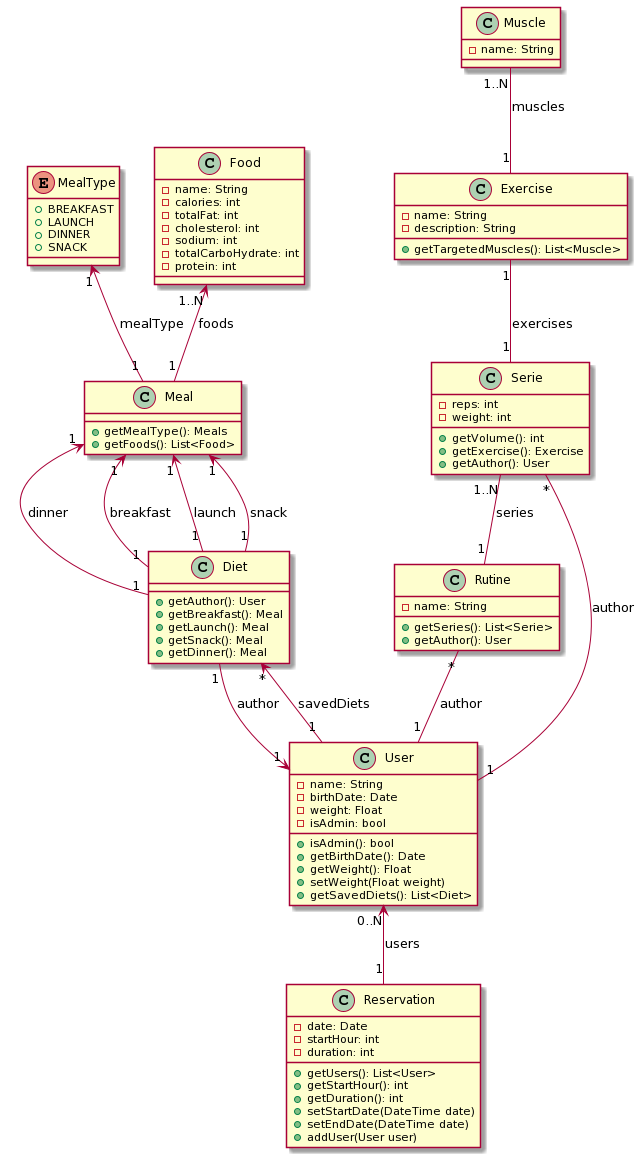
\includegraphics[width=0.6\textwidth]{uml}
	\caption{Diagrama UML}
\end{figure}

\newpage

\subsection{Diagrama Casos de Uso}

\begin{figure}[h]
 	\centering
	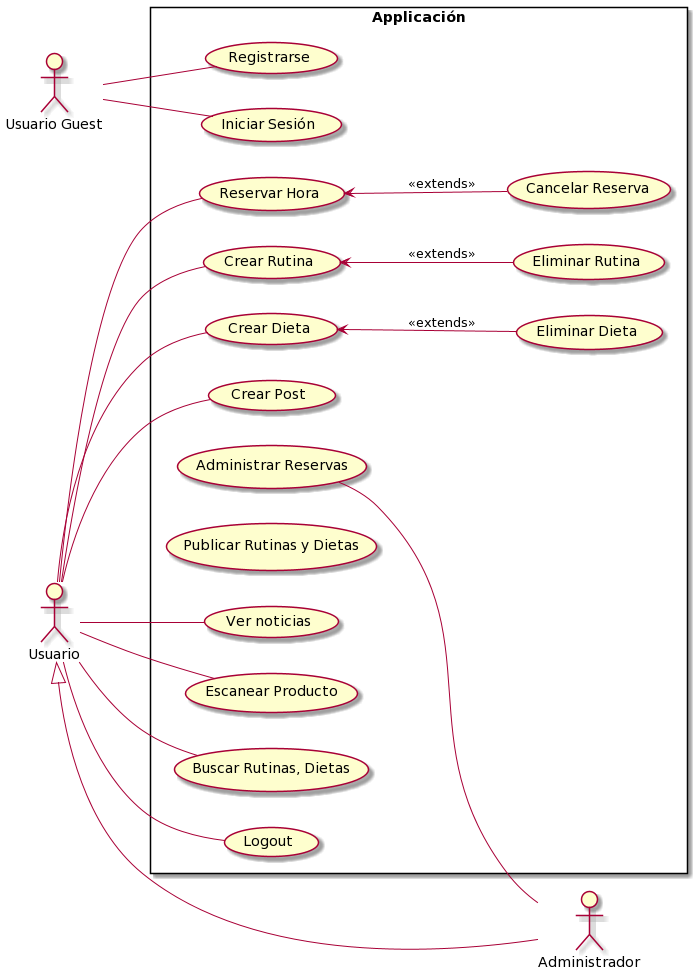
\includegraphics[width=0.6\textwidth]{casos_uso}
	\caption{Diagrama de Casos de Uso}
\end{figure}

TODO: Explicar casos de uso paso a paso. e.g: 1. seleccionar boton x, hacer x, etc

\newpage

\subsection{Diagrama Relacional (bases de datos)}

\begin{figure}[h]
 	\centering
	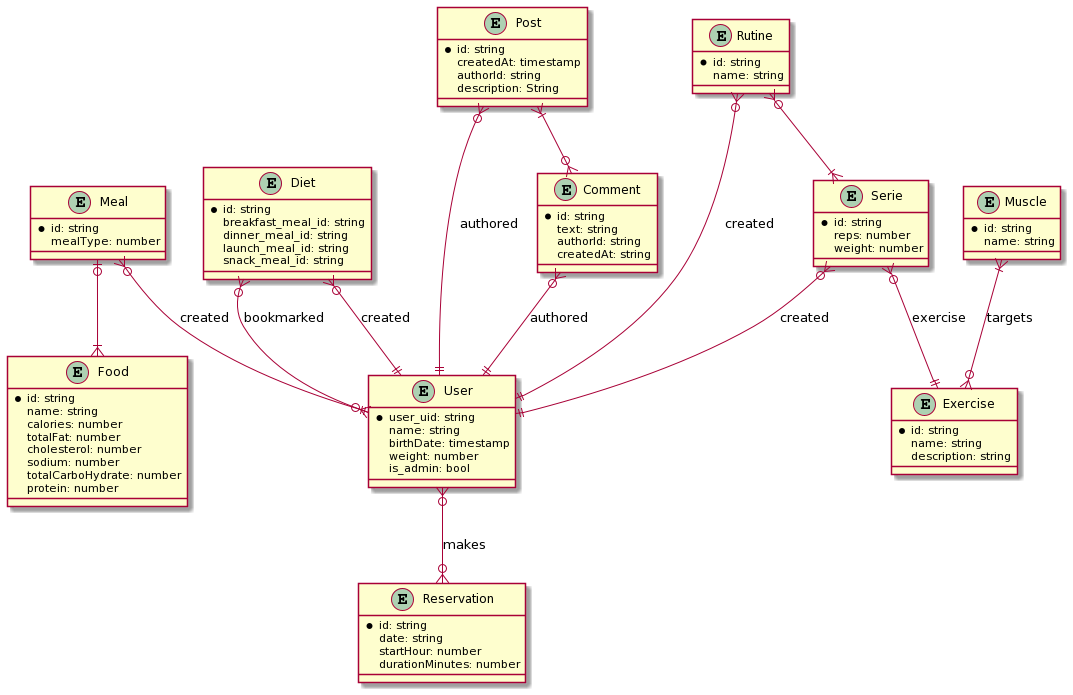
\includegraphics[width=0.6\textwidth]{diagramaer}
	\caption{Diagrama Entidad Relacion}
\end{figure}

\newpage

\section{Diseño}
TODO: Qué leyes de gestalt

El objetivo del diseño es dar al usuario una experiencia fluida y cómoda mientras hace uso de la aplicación, por lo que cada elemento se sitúa en lugares de la pantalla que el usuario encontrará intuitivo.
Además, se han hecho uso del contraste entre colores y varias leyes de Gestalt, tales como la ley de la simetría y la experiencia.

\subsection{Logo}
El logo se compone de un símbolo y texto; el símbolo es un brazo con cierta musculatura levatando una pesa, en este símobolo se puede advertir la forma de un corazón, dando a entender el amor por el \textit{fitness}.
El texto es el nombre de la aplicación usando nuestro color principal y la fuente \textbf{Montserrat} en negrita, el resto de la aplicación también hace uso de ésta.


\subsection{Colores}
TODO: explicar los colores utilizados

Los efectos del ejercicio en el ser humano son positivos; reduce el estrés, la asiedad y la depresión gracias a la segregación de \textbf{endorfinas}, unas sustancias químicas que producen sensación de felicidad y euforia.

Hemos querido representar esos efectos en nuestro diseño a través del color \textbf{naranja} como color principal, ya que, según la psicología del color, el naranja es energético que se asocia con juventud, alegría y dinamismo.
Para destacar nuestro color principal y hacer contraste, se han escogido colores oscuros y el blanco. Los colores se asocian con la fortaleza y el blanco con la paz y tranquilidad, efectos que se consiguen también al tener un vida con una actividad física presente.

\begin{figure}[h]
  \centering
 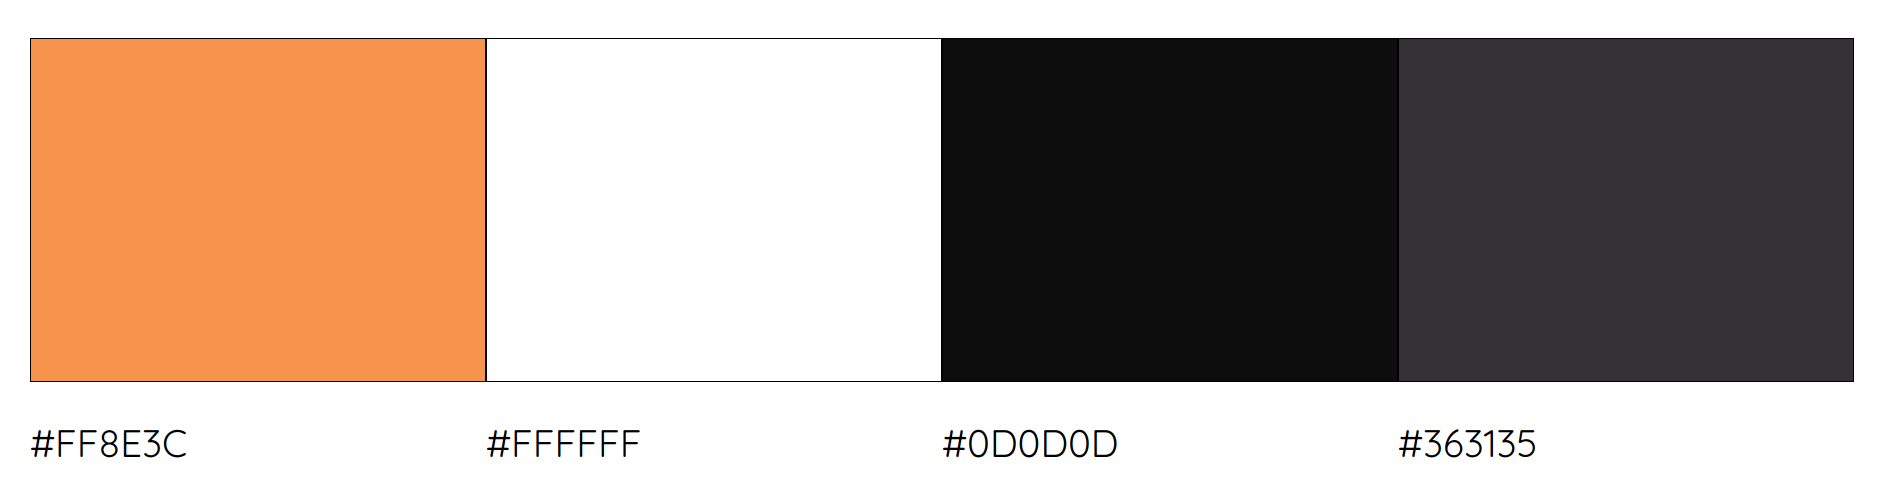
\includegraphics[width=1\textwidth]{color_palette}
 \caption{Paleta de colores}
\end{figure}



\subsection{Mockup}
\href{https://mockittapp.wondershare.com/app/3398ef738f7ac4f35fae5df4eb77004473612d19?simulator_type=device&sticky}{Link al mockup}

todo: poner foto

\newpage

\section{Estadísticas sobre el proyecto}
TODO: Alomejor no hace falta esta seccion pero: poner stats de git, lineas codigo etc

\newpage

\section{Conclusión}

\subsection{Posibles ampliaciones}
Todo: hacer

\end{document}